\begin{center}


	\tikzset{every picture/.style={line width=0.75pt}} %set default line width to 0.75pt        

	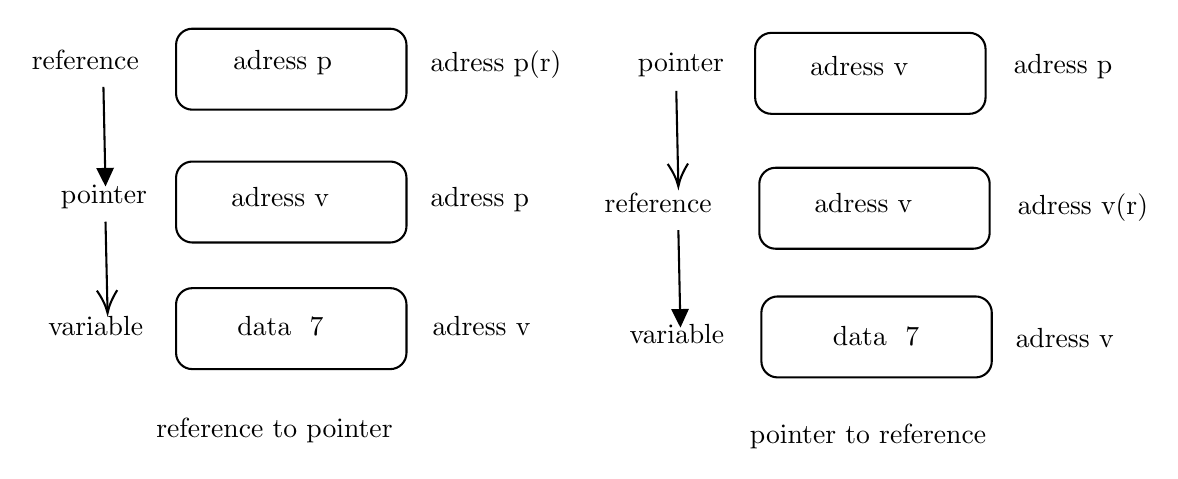
\begin{tikzpicture}[x=0.75pt,y=0.75pt,yscale=-1,xscale=1]
	%uncomment if require: \path (0,300); %set diagram left start at 0, and has height of 300
	
	%Rounded Rect [id:dp11927883071932444] 
	\draw   (85,185.8) .. controls (85,181.49) and (88.49,178) .. (92.8,178) -- (188.2,178) .. controls (192.51,178) and (196,181.49) .. (196,185.8) -- (196,209.2) .. controls (196,213.51) and (192.51,217) .. (188.2,217) -- (92.8,217) .. controls (88.49,217) and (85,213.51) .. (85,209.2) -- cycle ;
	%Rounded Rect [id:dp6640212087116251] 
	\draw   (85,124.8) .. controls (85,120.49) and (88.49,117) .. (92.8,117) -- (188.2,117) .. controls (192.51,117) and (196,120.49) .. (196,124.8) -- (196,148.2) .. controls (196,152.51) and (192.51,156) .. (188.2,156) -- (92.8,156) .. controls (88.49,156) and (85,152.51) .. (85,148.2) -- cycle ;
	%Rounded Rect [id:dp3237041947663375] 
	\draw   (85,60.8) .. controls (85,56.49) and (88.49,53) .. (92.8,53) -- (188.2,53) .. controls (192.51,53) and (196,56.49) .. (196,60.8) -- (196,84.2) .. controls (196,88.51) and (192.51,92) .. (188.2,92) -- (92.8,92) .. controls (88.49,92) and (85,88.51) .. (85,84.2) -- cycle ;
	%Rounded Rect [id:dp9477857736296029] 
	\draw   (367,189.8) .. controls (367,185.49) and (370.49,182) .. (374.8,182) -- (470.2,182) .. controls (474.51,182) and (478,185.49) .. (478,189.8) -- (478,213.2) .. controls (478,217.51) and (474.51,221) .. (470.2,221) -- (374.8,221) .. controls (370.49,221) and (367,217.51) .. (367,213.2) -- cycle ;
	%Rounded Rect [id:dp4721875816932608] 
	\draw   (366,127.8) .. controls (366,123.49) and (369.49,120) .. (373.8,120) -- (469.2,120) .. controls (473.51,120) and (477,123.49) .. (477,127.8) -- (477,151.2) .. controls (477,155.51) and (473.51,159) .. (469.2,159) -- (373.8,159) .. controls (369.49,159) and (366,155.51) .. (366,151.2) -- cycle ;
	%Rounded Rect [id:dp34593900558257906] 
	\draw   (364,62.8) .. controls (364,58.49) and (367.49,55) .. (371.8,55) -- (467.2,55) .. controls (471.51,55) and (475,58.49) .. (475,62.8) -- (475,86.2) .. controls (475,90.51) and (471.51,94) .. (467.2,94) -- (371.8,94) .. controls (367.49,94) and (364,90.51) .. (364,86.2) -- cycle ;
	%Straight Lines [id:da5154723980908134] 
	\draw    (51,146) -- (51.95,188) ;
	\draw [shift={(52,190)}, rotate = 268.7] [color={rgb, 255:red, 0; green, 0; blue, 0 }  ][line width=0.75]    (10.93,-4.9) .. controls (6.95,-2.3) and (3.31,-0.67) .. (0,0) .. controls (3.31,0.67) and (6.95,2.3) .. (10.93,4.9)   ;
	%Straight Lines [id:da5246033953497637] 
	\draw    (50,81) -- (50.94,126) ;
	\draw [shift={(51,129)}, rotate = 268.81] [fill={rgb, 255:red, 0; green, 0; blue, 0 }  ][line width=0.08]  [draw opacity=0] (8.93,-4.29) -- (0,0) -- (8.93,4.29) -- cycle    ;
	%Straight Lines [id:da36423552536908654] 
	\draw    (327,150) -- (327.94,194) ;
	\draw [shift={(328,197)}, rotate = 268.78] [fill={rgb, 255:red, 0; green, 0; blue, 0 }  ][line width=0.08]  [draw opacity=0] (8.93,-4.29) -- (0,0) -- (8.93,4.29) -- cycle    ;
	%Straight Lines [id:da2981001586744325] 
	\draw    (326,83) -- (326.96,127) ;
	\draw [shift={(327,129)}, rotate = 268.75] [color={rgb, 255:red, 0; green, 0; blue, 0 }  ][line width=0.75]    (10.93,-4.9) .. controls (6.95,-2.3) and (3.31,-0.67) .. (0,0) .. controls (3.31,0.67) and (6.95,2.3) .. (10.93,4.9)   ;
	
	% Text Node
	\draw (74,239) node [anchor=north west][inner sep=0.75pt]   [align=left] {reference to pointer};
	% Text Node
	\draw (360,242) node [anchor=north west][inner sep=0.75pt]   [align=left] {pointer to reference};
	% Text Node
	\draw (113,190) node [anchor=north west][inner sep=0.75pt]   [align=left] {data \ 7};
	% Text Node
	\draw (22,190) node [anchor=north west][inner sep=0.75pt]   [align=left] {variable};
	% Text Node
	\draw (207,190) node [anchor=north west][inner sep=0.75pt]   [align=left] {adress v};
	% Text Node
	\draw (28,127) node [anchor=north west][inner sep=0.75pt]   [align=left] {pointer};
	% Text Node
	\draw (206,128) node [anchor=north west][inner sep=0.75pt]   [align=left] {adress p};
	% Text Node
	\draw (14,62) node [anchor=north west][inner sep=0.75pt]   [align=left] {reference};
	% Text Node
	\draw (206,62) node [anchor=north west][inner sep=0.75pt]   [align=left] {adress p(r)};
	% Text Node
	\draw (111,62) node [anchor=north west][inner sep=0.75pt]   [align=left] {adress p};
	% Text Node
	\draw (110,128) node [anchor=north west][inner sep=0.75pt]   [align=left] {adress v};
	% Text Node
	\draw (290,131) node [anchor=north west][inner sep=0.75pt]   [align=left] {reference};
	% Text Node
	\draw (306,63) node [anchor=north west][inner sep=0.75pt]   [align=left] {pointer};
	% Text Node
	\draw (302,194) node [anchor=north west][inner sep=0.75pt]   [align=left] {variable};
	% Text Node
	\draw (488,196) node [anchor=north west][inner sep=0.75pt]   [align=left] {adress v};
	% Text Node
	\draw (400,195) node [anchor=north west][inner sep=0.75pt]   [align=left] {data \ 7};
	% Text Node
	\draw (487,64) node [anchor=north west][inner sep=0.75pt]   [align=left] {adress p};
	% Text Node
	\draw (489,131) node [anchor=north west][inner sep=0.75pt]   [align=left] {adress v(r)};
	% Text Node
	\draw (391,131) node [anchor=north west][inner sep=0.75pt]   [align=left] {adress v};
	% Text Node
	\draw (389,65) node [anchor=north west][inner sep=0.75pt]   [align=left] {adress v};
	
	
	\end{tikzpicture}
\end{center}